\documentclass[12pt]{article}
\usepackage{amsmath}
\usepackage{amssymb}
\usepackage{amsthm}
\usepackage{accents}
\usepackage{graphicx}
\setlength{\oddsidemargin}{0in}
\setlength{\textwidth}{6.5in}
\setlength{\topmargin}{-.55in}
\setlength{\textheight}{9in}
\pagestyle{empty}
\renewcommand \d{\displaystyle}
\begin{document}
\noindent Dallas Klumpe

\noindent Math 5820

\noindent HW 18

11.3.2.a. The best straight line through the Massachusetts funding/graduation rate data has the equation $y=81.088+0.412x$, where $s=11.78848$. Construct a $95\%$ confidence interval for $\beta_1$.\\
Well, given the data, we have that $\sum_{i=1}^26(x_i-\bar{x})^2=\sum_{i=1}^26x_i^2-n\bar{x}^2=5365.08-26(13.84615)^2=380.4646$. Now, $t_{\alpha/2}=2.0639$. So, our confidence interval is $[0.412-2.0639(\frac{11.78848}{\sqrt{380.4646}}), 0.412+2.0639(\frac{11.78848}{\sqrt{380.4646}})]=[-0.83535, 1.65935]$.\\
b. What does this answer imply about the outcome of testing $H_0:\beta_1=0$ versus $H_1:\beta_1\neq0$ at the $\alpha=0.05$ level of significance?\\
Since we see that $0\in[-0.83535, 1.65935]$, we fail to reject $H_0$ at the $0.05$ level of significance.\\
c. Graph the data and superimpose the regression line. How would you summarize these data, and their implications, to a meeting of the state School Board?\\
Well, given the data, the fact that $0\in[-0.83535, 1.65935]$ at the $0.05$ significance level, and the graph below, we can say with $95\%$ confidence that there is a neutral correspondance between spending per student and graduation rate. That is, there is significant increase or decrease in graduation rates with respect ot an increase in spending per student.
\begin{center}
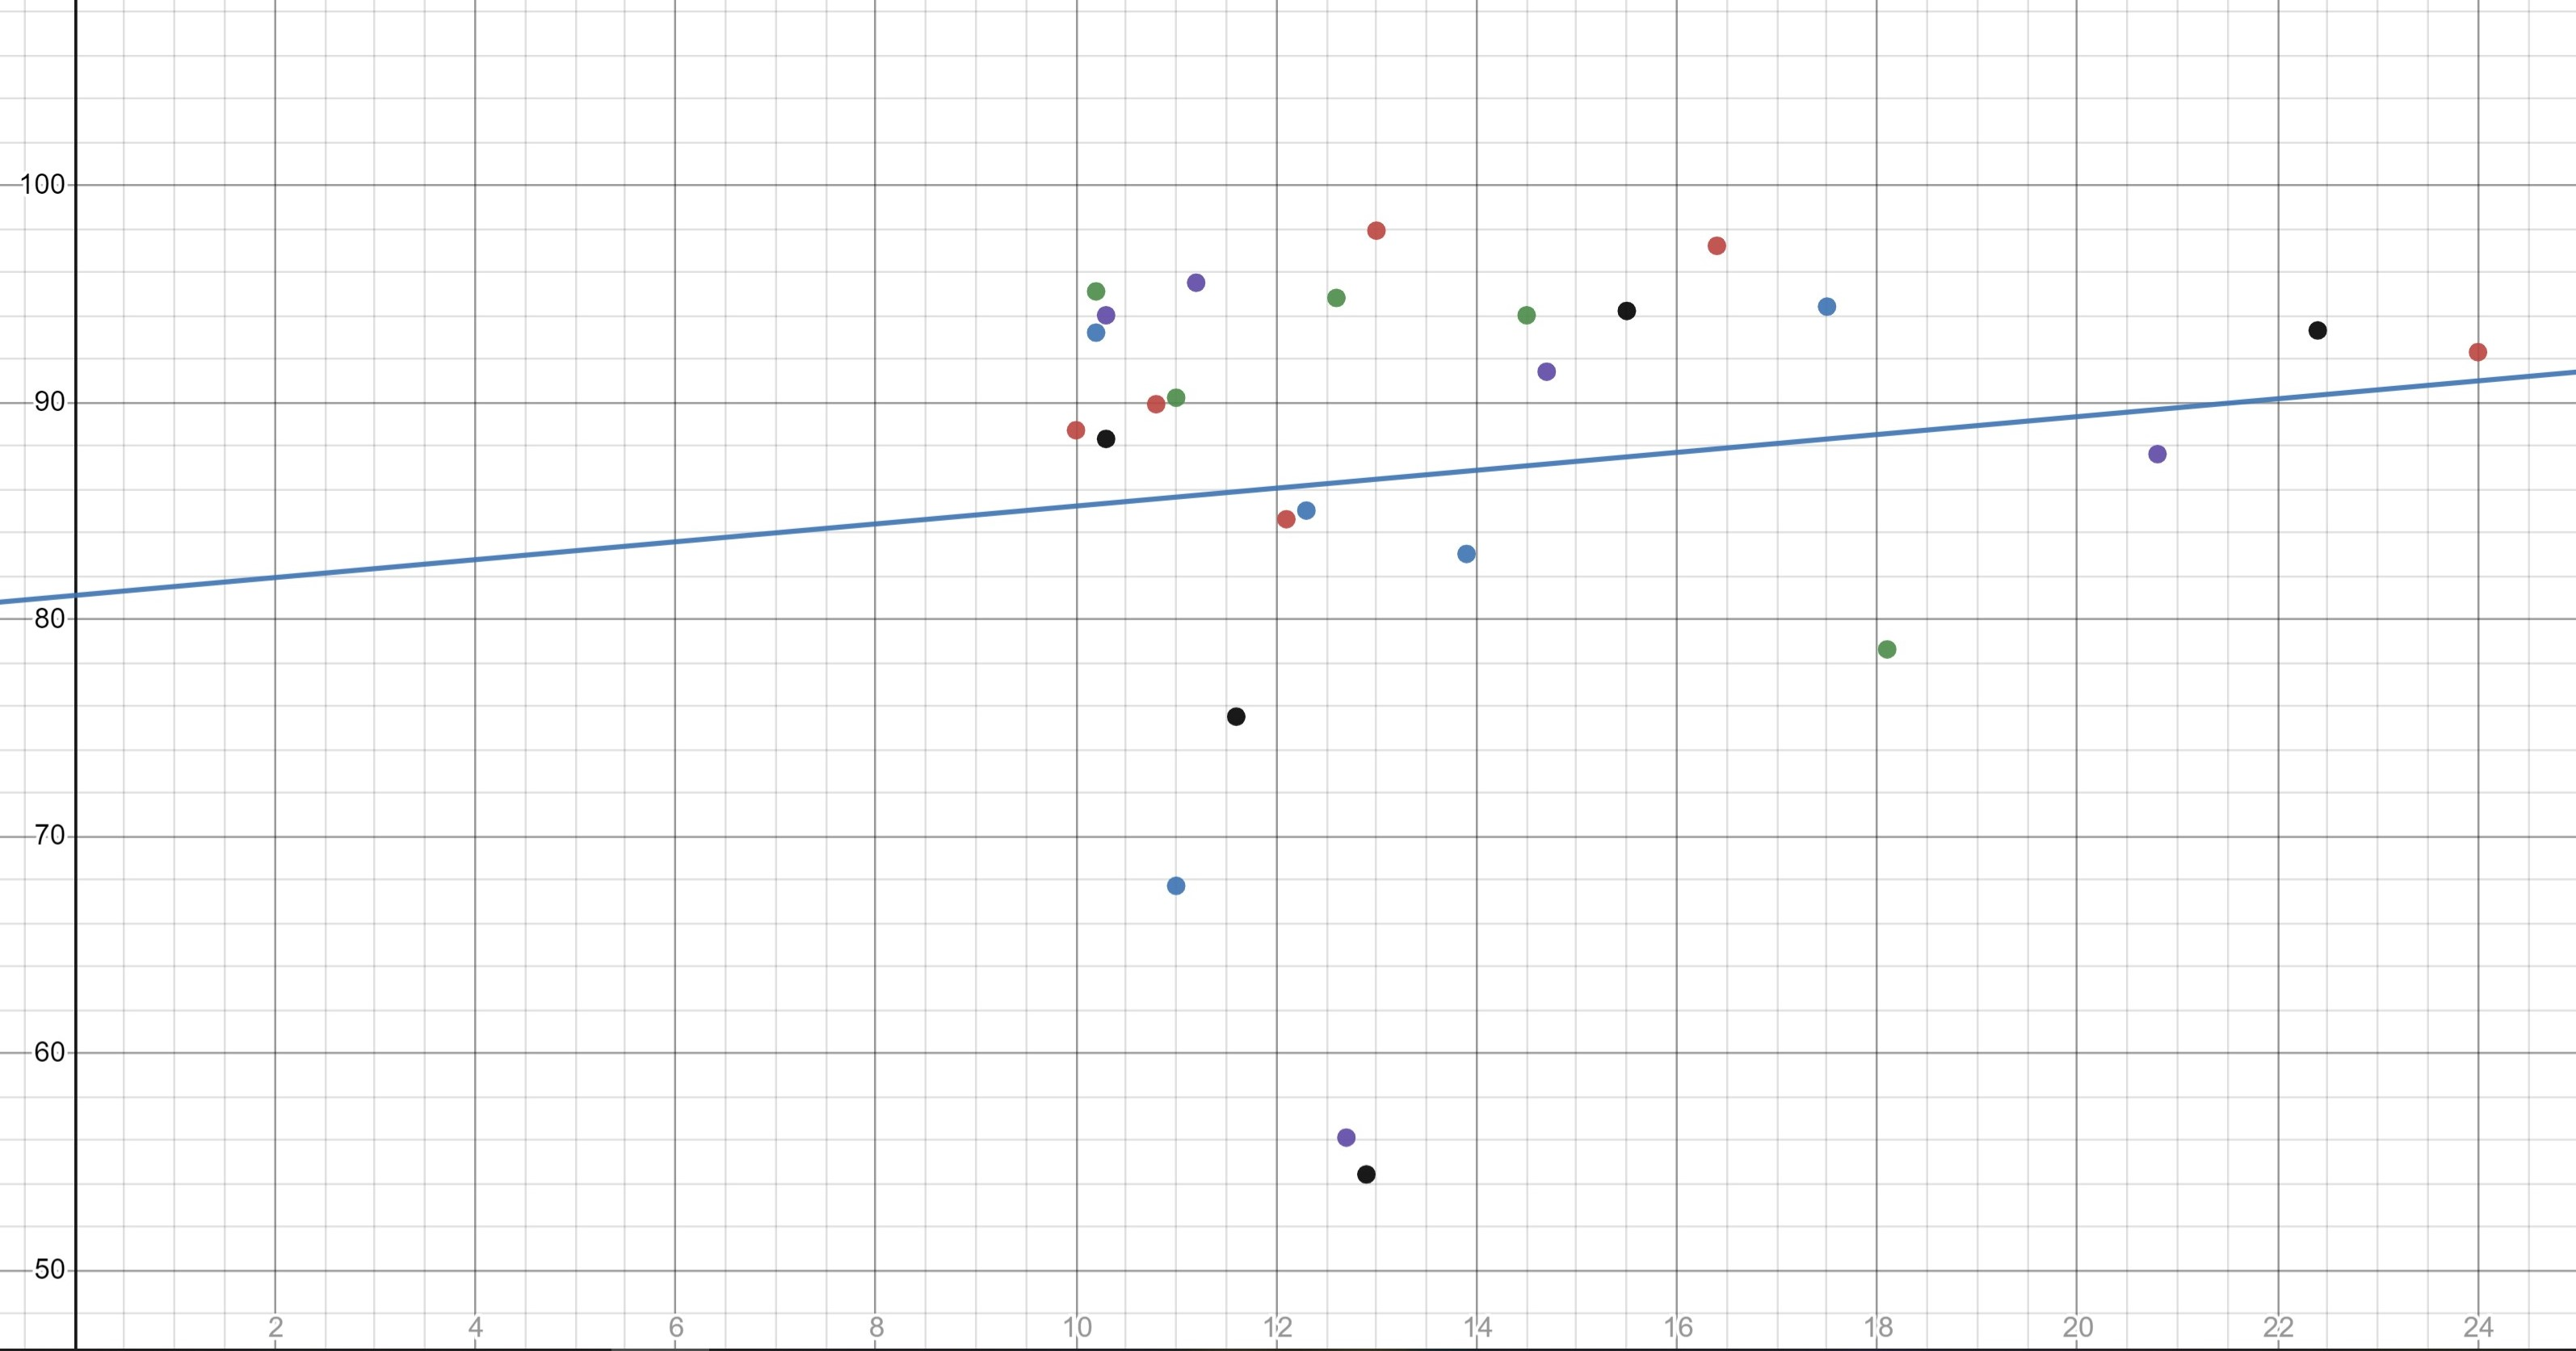
\includegraphics[scale=0.4]{11-3-2.JPG}\\[20pt]
\end{center}

11.3.9. Test $H_0:\beta1=0$ versus $H_1:\beta_1\neq0$ for the plumage index/behavioral index data given in Question 11.2.11. Let $\alpha=0.05$. Use the fact that $y=0.61+0.84x$ is the best straight line describing the xy-relationship.\\
Given the data, we have that $s^2=5.7797$. Hence, $s=\sqrt{5.7797}=2.4041$. Also given the data, we have that $\sum_{i=1}^{11}(x_i-\bar{x})^2=156.9091$. Now, $t_{\alpha/2}=2.2622$. So, $t=\frac{0.84}{\frac{2.4041}{\sqrt{156.9091}}}=4.3767$. Since $t>t_{\alpha/2}$, we reject $H_0$ at $95\%$ significance.\\[20pt]

11.3.13. State the decision rule and the conclusion if $H_0:\sigma^2=12.6$ is to be tested against $H_1:\sigma^2\neq12.6$ where $n=24, s^2=18.2$, and $\alpha=0.05$.\\
Well, $\chi^2_{1-\alpha/2}=36.781$ and $\chi^2_{\alpha/2}=10.982$. We will fail to reject $H_0$ if $10.982<\chi^2<36.781$. Now, $\chi^2=\frac{22*18.2}{12.6}=31.7778$. Since $10.982<31.7778<36.781$, we do indeed fail to reject $H_0$.




\end{document}